\section{Agents' Welfare}\label{app:welfare}
Figure~\ref{fig:SW-regions} highlights the change in utility when agents are behaviorally biased (vs. when they were rational) across different regions in the feature space, with the regions generated based on the firm's optimal choice of threshold and agents' responses to it. In particular, the utility of agents in the green-highlighted region (this is $\sY(\vtheta_\text{B}, \theta_{0,\text{B}}) \cap \sN(\vtheta_\text{NB}, \theta_{0,\text{NB}})$ in Proposition~\ref{prop:mismatch-actual-b}) increases when they are behaviorally biased. One subset of agents in this region are those 
%$\sY(\vtheta_\text{B}, \theta_{0,\text{B}}) \cap \sN(\vtheta_\text{NB}, \theta_{0,\text{NB}})\cap \sA(\vtheta_\text{NB}, \theta_{0, \text{NB}})$ where 
who in the rational case exert effort to get admitted and have a utility $r-c(\vx,\vx_0)$, whereas in the behaviorally biased case they attain utility $r > r-c(\vx,\vx_0)$ as they get admitted without any effort (and they correctly assume so). Another one is %subset is $(\sY(\vtheta_\text{B}, \theta_{0,\text{B}}) \cap \sN(\vtheta_\text{NB}, \theta_{0,\text{NB}}))/\sA(\vtheta_\text{NB}, \theta_{0,\text{NB}})$ which is 
the subset of agents who would not try to get to the decision boundary in the rational case (and so have utility of $0$), but in the behavioral case, they are receiving utility $r$ without any movement and due to the change of the decision boundary. For the numerical example in the bottom row of Figure~\ref{fig:firm-benefit-hurt-dist}, there are more agents in this green-highlighted region than in the remaining red-highlighted regions (where biased agents have lower utility than rational agents), leading to an overall higher welfare for all agents when they are biased compared to when they were rational. 

\begin{figure}[ht]
    \centering
    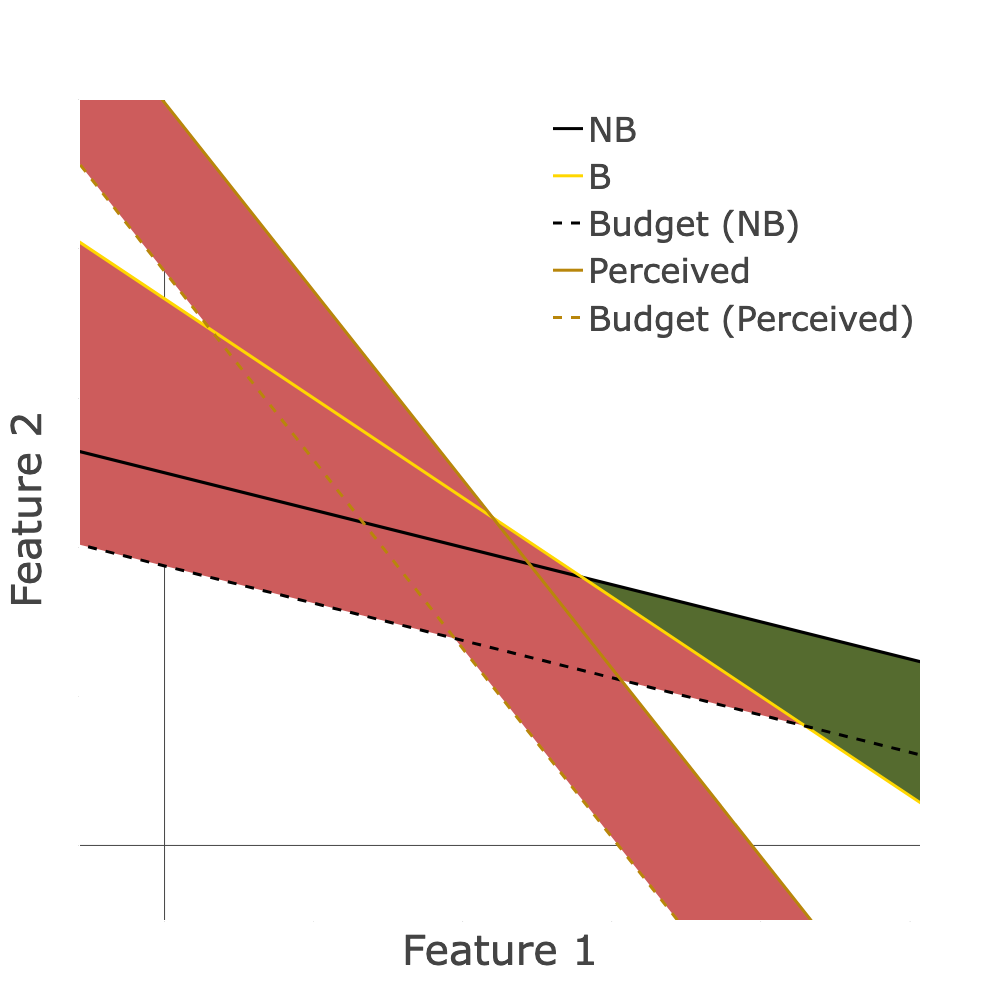
\includegraphics[width=0.4\linewidth]{Figures/SW_highlighted regions.png}
    \caption{Regions where agents have higher (green) or lower (red) utility when biased vs. when rational.}
    \Description[Welfare regions]{Regions where agents have higher (green) or lower (red) utility when biased vs. when rational.}
    \label{fig:SW-regions}
\end{figure}